\section{\protect\uppercase{Model}}

% \input{Sections/Model_Specimen}
% \input{Sections/Model_Material}
\subsection{Discretization}

A FE based mesh input is used by Peridigm. As it is expected there are differences in the choice of the horizon and element size for structured and unstructured based meshes, both are considered here. The specimen creation in a versatile parametric model generator allows for a quick change of the underlying discretization scheme and the element size. The base FE models and resulting PD discretizations are shown in \autoref{fig:Model:Discretization}.


% Styles
\tikzset{
  modelspy style/.style={
    spy scope={%
      modelspyscope style,%
    },
    connect spies/.style={
      modelspyconnect style,%
    },
  }
}

\tikzset{
  modelspyscope style/.style={
    magnification=4,
    connect spies,                            % Connect orig. & detail
    width=0.3\linewidth,                      % Spy width
    height=0.2\linewidth,                    % Spy height
    every spy on node/.style={                % Source
      rectangle,                              % Form
      rounded corners=0.01\linewidth,         % Edge shape
      dashed,                                 % Dashed line
      draw=black,                             % Line color
      %thick,                                  % Line style for spy
    },
    every spy in node/.style={                % Spy
      rectangle,                              % Form
      rounded corners=0.04\linewidth,         % Edge shape
      dashed,                                 % Dashed line
      draw=black,                             % Line color
      %thick,                                  % Line style for spy
    },
  },
}

\tikzset{
  modelspyconnect style/.style={
    spy connection path={
      \draw[%
        %thick,
        dashed,
        black
      ] (tikzspyonnode) -- (tikzspyinnode); % In-On-Connection
    },
  },
}
% Hex:
\begin{figure}[htbp]
  \begin{subfigure}{0.49\linewidth}
    \centering
    %\includegraphics[width=\linewidth,height=4cm,keepaspectratio]{../../Material/Figures/Model_FE_Hex_0-4_ct}
    %\includegraphics[width=\linewidth,height=4cm,keepaspectratio]{Model_FE_Hex_0-4_ct}
    \tikzexternalenable
    \tikzsetnextfilename{Model_FE_Hex_0-4_ct}
    \begin{tikzpicture}[modelspy style]
      \node[anchor=south west,inner sep=0] (image) at (0,0) {\includegraphics[width=\linewidth,height=4cm,keepaspectratio]{Model_FE_Hex_0-4_ct}};
      \begin{scope}[
        shift={(image.south west)},
        x={(image.south east)},
        y={(image.north west)},
      ]
        \coordinate (spypointfehex) at (0.825,0.740);
        \coordinate (spyviewerfehex) at (0.80,0.25);
        \spy on (spypointfehex) in node at (spyviewerfehex);
      \end{scope}
    \end{tikzpicture}
    \tikzexternaldisable
    \caption{Base hex FE mesh}
    \label{fig:Model:Discretization:Hex:FE}
  \end{subfigure}%
  \hfill
  \begin{subfigure}{0.49\linewidth}
    \centering
    %\includegraphics[width=\linewidth,height=4cm,keepaspectratio]{../../Material/Figures/Model_PD_Hex_0-4_ct}
    %\includegraphics[width=\linewidth,height=4cm,keepaspectratio]{Model_PD_Hex_0-4_ct}
    \tikzexternalenable
    \tikzsetnextfilename{Model_PD_Hex_0-4_ct}
    \begin{tikzpicture}[modelspy style]
      \node[anchor=south west,inner sep=0] (image) at (0,0) {\includegraphics[width=\linewidth,height=4cm,keepaspectratio]{Model_PD_Hex_0-4_ct}};
      \begin{scope}[
        shift={(image.south west)},
        x={(image.south east)},
        y={(image.north west)},
      ]
        \coordinate (spypointpdhex) at (0.825,0.740);
        \coordinate (spyviewerpdhex) at (0.80,0.25);
        \spy on (spypointpdhex) in node at (spyviewerpdhex);
      \end{scope}
    \end{tikzpicture}
    \tikzexternaldisable
    \caption{PD representation of hex mesh}
    \label{fig:Model:Discretization:Hex:PD}
  \end{subfigure}%
  \\
%   \caption{Structured discretization}
%   \label{fig:Model:Discretization:Hex}
% \end{figure}
% 
% Tet:
% 
% \begin{figure}[htbp]
  \begin{subfigure}{0.49\linewidth}
    \centering
    %\includegraphics[width=\linewidth,height=4cm,keepaspectratio]{../../Material/Figures/Model_FE_Tet_0-67_ct}
    %\includegraphics[width=\linewidth,height=4cm,keepaspectratio]{Model_FE_Tet_0-67_ct}
    \tikzexternalenable
    \tikzsetnextfilename{Model_FE_Tet_0-67_ct}
    \begin{tikzpicture}[modelspy style]
      \node[anchor=south west,inner sep=0] (image) at (0,0) {\includegraphics[width=\linewidth,height=4cm,keepaspectratio]{Model_FE_Tet_0-67_ct}};
      \begin{scope}[
        shift={(image.south west)},
        x={(image.south east)},
        y={(image.north west)},
      ]
        \coordinate (spypointfetet) at (0.825,0.740);
        \coordinate (spyviewerfetet) at (0.80,0.25);
        \spy on (spypointfetet) in node at (spyviewerfetet);
      \end{scope}
    \end{tikzpicture}
    \tikzexternaldisable
    \caption{Base tet FE mesh}
    \label{fig:Model:Discretization:Tet:FE}
  \end{subfigure}%
  \hfill
  \begin{subfigure}{0.49\linewidth}
    \centering
    %\includegraphics[width=\linewidth,height=4cm,keepaspectratio]{../../Material/Figures/Model_PD_Tet_0-67_ct}
    %\includegraphics[width=\linewidth,height=4cm,keepaspectratio]{Model_PD_Tet_0-67_ct}
    \tikzexternalenable
    \tikzsetnextfilename{Model_PD_Tet_0-67_ct}
    \begin{tikzpicture}[modelspy style]
      \node[anchor=south west,inner sep=0] (image) at (0,0) {\includegraphics[width=\linewidth,height=4cm,keepaspectratio]{Model_PD_Tet_0-67_ct}};
      \begin{scope}[
        shift={(image.south west)},
        x={(image.south east)},
        y={(image.north west)},
      ]
        \coordinate (spypointpdtet) at (0.825,0.740);
        \coordinate (spyviewerpdtet) at (0.80,0.25);
        \spy on (spypointpdtet) in node at (spyviewerpdtet);
      \end{scope}
    \end{tikzpicture}
    \tikzexternaldisable
    \caption{PD representation of tet mesh}
    \label{fig:Model:Discretization:Tet:PD}
  \end{subfigure}%
%   \caption{Unstructured discretization}
%   \label{fig:Model:Discretization:Tet}
  \caption{Discretization schemes and PD representation}
  \label{fig:Model:Discretization}
\end{figure}

The structured mesh is doubly symmetric regarding the specimen $x$-$y$- as well as the $x$-$z$-plane. The unstructured meshes are only symmetric about the $x$-$z$-plane.

Especially in higher dimensions, the horizon cannot be too large either as this results in the boundary layer, where displacement boundary conditions are imposed, being the majority of the simulation domain \cite{SelesonP2016b}. Thus, a no-damage zone (red) is introduced in the vicinity of the specimen ends. In this region failure is not modeled to avoid effects of the boundary conditions on the failure behavior. Based on the findings in the experiments this approach is valid.



\subsection{Loads and boundary conditions}

Both specimen ends are clamped in the test fixture. The tensile experiments are strain-controlled by means of a constant velocity on one of the clamping regions. The homogeneous displacement and inhomogeneous velocity boundary conditions are applied on respective node sets at the specimen ends. As these sets are defined on the base FE mesh, there is a small deviation of the application region in the PD model. This has no effect on the results. Various combinations of displacement boundary conditions were investigated. The influence on the results is negligible.

% BC:

\begin{figure}[htbp]
  \begin{subfigure}{0.49\linewidth}
    \centering
    %\includegraphics[width=\linewidth,height=4cm,keepaspectratio]{../../Material/Figures/Model_Mix_Hex_0-4_BC_NodeSets_Iso_ct}
    \includegraphics[width=\linewidth,height=4cm,keepaspectratio]{Model_Mix_Hex_0-4_BC_NodeSets_Iso_ct}
    \caption{Iso view}
    \label{fig:Model:Discretization:LBC:Iso}
  \end{subfigure}%
  \hfill
  \begin{subfigure}{0.49\linewidth}
    \centering
    %\includegraphics[width=\linewidth,height=4cm,keepaspectratio]{../../Material/Figures/Model_Mix_Hex_0-4_BC_NodeSets_ct}
    \includegraphics[width=\linewidth,height=4cm,keepaspectratio]{Model_Mix_Hex_0-4_BC_NodeSets_ct}
    \caption{Detail of FE (blue) and PD (green) node set}
    \label{fig:Model:Discretization:LBC:Detail}
  \end{subfigure}%
  \caption{Constraint and load introduction domains}
  \label{fig:Model:Discretization:LBC:Tet}
\end{figure}

% Boundary conditions: \cite{MadenciE2016} f�r ``richtige'' Randbedingungen nicht angewendet, aber Bereich Randbedingungen weit genug weg, sodass kein Einfluss R�nder auf Versagen

Madenci and Oterkus \cite{MadenciE2016} point out, that simply imposing constant boundary condition values on a material regions leads to incorrect behavior of the actual boundary and the domain within a distance of one horizon from the application region. A modified approach to reflect the correct boundary conditions is proposed but not used here as the no-failure-zone in the model is large enough to smooth boundary effects.

% \FloatBarrier





% Vorteile der Stochastic (Ziel):
% 
% \begin{itemize}
%   \item Wiedergabe der inhomogenen Materialstruktur (siehe Bild Jochen)
%   \item Abschw�chung von Effekten der Diskretisierung
%   \item \cite{JeonBS2015} for modelling crack propagation, an initial flaw is highly suggested $\rightarrow$ Steifigkeitsunterschied kann als initialer Schaden angesehen werden
% \end{itemize}


% \subsection{Format}
% 
% The first page must contain the Title, Author(s), Affiliation(s), Key words and the Summary. The Introduction must begin immediately below, following the format of this template.
% 
% \subsubsection{Title}
% The title should be written with all capital letters.
% \subsubsection{Author}
% The author's name should include first name, middle initial and surname.
% \subsubsection{key words}
% Please, write no more than three keywords.
% 
% \subsection{Figures}
% 
% Figures are automatically numbered consecutively and captioned, and should be embedded in the Paper, see for example Figure~\ref{fig:natlab}.
% 
% \begin{figure}[!h]
%  \centering\includegraphics[width=0.5\linewidth]{example-image-a}
%  \caption{The former Philips research centre NatLab, which is the venue of this conference.}
%  \label{fig:natlab}
% \end{figure}
% 
% \subsection{Equations}
% 
% A displayed equation is automatically numbered, using Arabic numbers in parentheses.
% The following example is a single line equation:
% 
% \begin{align}
%  Ax = b
% \end{align}
% 
% The next example is a multi-line equation:
% \begin{equation}
%  \begin{aligned}
%   Ax &=b \\
%   Ax &=b
%  \end{aligned}
% \end{equation}
% 
% \subsection{Tables}
% 
% All tables are automatically numbered consecutively and captioned.
% 
% \begin{table}[!h]
% \centering
% \setlength{\arrayrulewidth}{2\arrayrulewidth}
% \begin{tabular}{ccc}
% \hline
% C11 & C12 & C13 \\
% C21 & C22 & C23 \\
% C31 & C32 & C33 \\
% C41 & C42 & C43 \\
% C51 & C52 & C53 \\
% \hline
% \end{tabular}
% \caption{Example of the construction of a table.}
% \end{table}
% 
% \subsection{Format of references}
% 
% References should be quoted in the text by numbers \cite{Barbero,Pimenta} and grouped together at the end of the Abstract in numerical order as shown in these instructions. Use the $unsrt$ style either with the $BibTeX$ or the $\backslash$$bibitem$ format.